\section{Molecular dynamics}
\label{Sec:MD}

FHI-aims provides the capability to run Born-Oppenheimer molecular
dynamics. The necessary keywords are described in this section. A
brief description of the physical algorithms implemented in FHI-aims
can be found in Ref. \cite{Blum08}. For a truly thorough explanation
of the underlying concepts, please refer to the standard literature,
e.g., Refs. \cite{frenkelsmit,bondjcompphys1999}.

\subsection*{Wave function extrapolation}

For molecular dynamics runs within the microcanonical ensemble (``$NVE$'') or
for deterministic thermostats, the wave function can be extrapolated in order
to reduce the computational effort to reach self-consistency.  This section
specifies \emph{what} quantity is actually extrapolated and \emph{how}.

Following the approach of K\"uhne \emph{et al.}  \cite{Kue07}, we extrapolate
the contra-covariant density matrix $\mathbf P \mathbf S$, the product of the
ordinary (purely contravariant) one-particle density matrix $\mathbf P$ and
the overlap matrix $\mathbf S$.  The contra-covariant density matrix is then
used to project new wave function coefficients from the last iteration
$\mathbf c_{\mathrm{new}} = (\mathbf P \mathbf S)_{\mathrm{extra}} \mathbf
c_{\mathbf{old}}$.  As a last step, the one-particle coefficients are
orthonormalized.

\begin{figure}[hb]
  \centering
  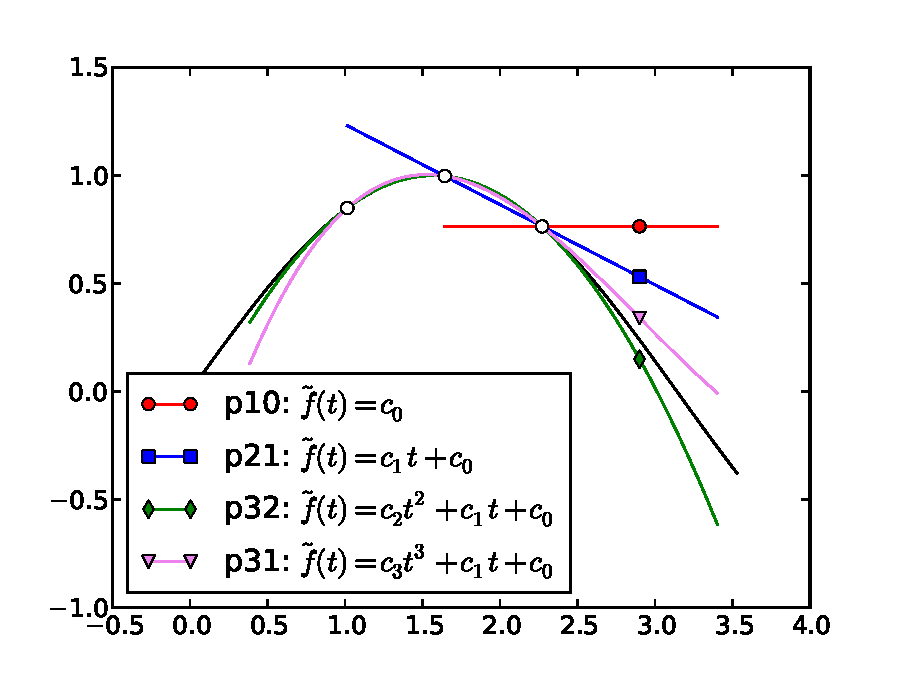
\includegraphics[width=0.7\textwidth]{extra}
  \caption{Different extrapolation schemes.  The scheme ``p$no$'' refers to an
    $n$ point scheme of order $o$, remaining orders used to fit odd
    components.}
  \label{fig:wf_extra-pno}
\end{figure}
The extrapolation scheme we use is sketched in Fig.~\ref{fig:wf_extra-pno} for
the example of an ordinary function $f(t)$ in a real variable $t$.  For a
p$no$ scheme (chosen with \keyword{wf\_extrapolation} \option{polynomial $n$
  $o$}) $n$ old iterations $f(t_0-k\Delta t)$, $k=1,\dotsc, n$ are stored.  An
ansatz function with $n$ degrees of freedom is then used to fit all of these
previous iterations and evaluated at $t_0$ and the value used to intialize the
SCF procedure.

The choice of the fitting function should aim at two targets: accurate
extrapolation and time-reversal symmetry.  The parameter $o$ specifies the
order of the extrapolation.  The higher $o$, the better the extrapolation gets
with decreasing time stemps $\Delta t$.  Time-reversal symmetry is useful to
avoid energetic drifts for not-so-tight SCF accuracy settings.  By adding odd
terms (odd with respect to $t_0+t \leftrightarrow t_0-t$), time-reversal
symmetry is enhanced \cite{Kolafa96-HOTR}.

Therefore, in contrast to \cite{Pulay04-FMD,Herbert-HG05-FMD}, the $(n-o-1)$
remaining degrees of freedom are not resolved within a least-squares fit but
instead to add fitting functions $(t-t_0)^{2k+1}$ to enhance time-reversal
symmetry and thus energy conversion.  Please note, however, that time-reversal
symmetry itself only enhances energy conservation and not necessarily
dynamical properties of the trajectories.

If you are interested in energy conservation, ``p31'' is in general a good
choice to start with.  If a good initial guess for the SCF procedure is
desired, you should give ``p32'' a try.  Please note that deactivation of
extrapolation (\keyword{wf\_extrapolation} \option{none}) is actually the same
as the ``p10'' extrapolation (see Fig.~\ref{fig:wf_extra-pno}) and simply uses
the one-particle coefficients of the last iteration are to initialize the SCF
procedure.


% \newpage

\subsection*{Tags for \texttt{geometry.in}:}

\keydefinition{velocity}{geometry.in}
{	\noindent
  Usage: \keyword{velocity} \option{vx} \option{vy} \option{vz} \\[1.0ex]
  Purpose: Specifies an initial velocity for the immediately preceding
    \keyword{atom} in file \texttt{geometry.in}. \\[1.0ex]
  \option{vx}, \option{vy}, \option{vz} : $x$, $y$, and $z$ components
    of the initial velocities, in \AA/ps. 
}
In \texttt{geometry.in}, the line containing the velocity must follow
the line containing the \keyword{atom} that the velocity refers
to. Note that, as in the case of relaxations, the molecular dynamics
section of the FHI-aims output stream contains this information in the
proper format.

\newpage

\subsection*{Tags for general section of \texttt{control.in}:}

\keydefinition{MD\_maxsteps}{control.in}
{\noindent
	Usage: \keyword{MD\_maxsteps} \option{N} \\[1.0ex]
	Purpose: Sets the maximal number of molecular dynamics
          steps. \\[1.0ex]
        \option{N} is an integer number. Default: -1 (infinite
          run). \\ 
}
A negative number signals that the ending criterion is not checked, in
fact, the default setting is \option{N}=-1. 

\keydefinition{check\_MD\_stop}{control.in}
{\noindent
      Usage: \keyword{check\_MD\_stop} \option{.true. / .false.}\\[1.0ex]
      Purpose: if \option{.true.}, an MD calculation ist stopped when a file MD\_stop is generated \\[1.0ex]
      Default: \option{.true.} \\}

\keydefinition{MD\_MB\_init}{control.in}
{\noindent
	Usage: \keyword{MD\_MB\_init} \option{Temperature} \\[1.0ex]
	Purpose: Initializes random velocities in a molecular dynamics calculation 
          using a Maxwell-Boltzmann distribution. \\[1.0ex]
        \option{Temperature} : Initial temperature in K. Default: No
          initial velocities. \\
}
This keyword is for a rough initialization only, and is overridden by
any successful calls of the MD restarting procedure through
\keyword{MD\_restart}. The default initialization for all velocities
is zero. 

\keydefinition{MD\_clean\_rotations}{control.in}
{\noindent
      Usage: \keyword{MD\_clean\_rotations} \option{.true. / .false.}\\[1.0ex]
      Purpose: if \option{.true.}, uses Sayvetz conditions to clean initial velocities from rotations\\[1.0ex]
      Default: \option{.true.} for non-periodic systems, \option{.false.} for
      periodic systems or if relaxation\_constraints are used.\\} 
This option is useful for non-periodic systems, allowing to weed out some
residual numerical noise in the forces. However, seeming rotations of the unit
cell can easily appear in periodic systems for completely normal, physical
reasons. Since this led to some confusion, this option is now actively
disabled (code stops) for periodic systems. If you have a good reason to use
this option in periodic systems, it can be re-introduced by hand.

\keydefinition{MD\_thermostat\_units}{control.in}
{\noindent
  Usage: \keyword{MD\_thermostat\_units} \option{units} \\[1.0ex]
  Purpose: To allow user specification of the effective thermostat
  mass outside of the internal units. \\[1.0ex]
  \option{unit} : Unit of the effective mass of the Nos\'e-Hoover and
    Nos\'e-Poincar\'e thermostats --
    either \option{amu*bohr\^{ }2} (mass-oriented specification) or
    \option{cm\^{ }-1} (frequency oriented specification, to
    allow to connect the thermostat mass to characteristic frequencies
    of the system). Default: \option{amu*bohr\^{ }2} . \\}

\keydefinition{MD\_restart}{control.in}
{\noindent
        Usage: \keyword{MD\_restart} \option{option} \\[1.0ex]
        Purpose: controls the MD initialization from a molecular
          dynamics restart file. \\[1.0ex]
        Restriction: At present, this keyword does not produce proper results
          when switching ensembles between runs. \\[1.0ex]  
        \option{option} is a string (see below). Default:
          \texttt{.false.} \\
} 
Possible values for \option{option} are \option{.true.}, \option{.false.}, 
\option{time\_restart}, or \option{filename}. The default is \option{.false.}. 

The data for the molecular dynamics integrator is always written to a file  
\option{aims\_MD\_restart.dat} after each time step (regardless of whether or
not keyword \keyword{MD\_restart} is used). 
If \keyword{MD\_restart} is set, this keyword controls the reading of such
data from a previous run (if that exists), to either 
\begin{itemize}
  \item continue a previous run (\option{.true.}), or
  \item to use previous position / velocity information
    but reset all timings (\option{time\_restart}), or
  \item to begin a new run from scratch (\option{.false.})
\end{itemize} 
The default file name is used unless the user specifies a 
specific file \option{filename} from where the input is to be read. 

\textbf{Important: If the starting structure and velocities are taken from 
the restart file, any exact positions noted in \option{geometry.in} are
ignored.} However, the species identification, possible initial charges, and
other per-atom information in \texttt{geometry.in} remain valid and must be
present as always. If the option \option{.true.} 
is set, the molecular dynamics clock is also read from file, in all 
other restarts the clock is reset to zero. 

\keydefinition{MD\_restart\_binary}{control.in}
{\noindent
        Usage: \keyword{MD\_restart\_binary} \option{option} \\[1.0ex]
        Purpose: controls the format used for the molecular
          dynamics restart file. \\[1.0ex]
        \option{option} is a string (see below). Default:
          \texttt{.true.} \\
} 
Possible values for \option{option} are \option{.true.} and \option{.false.}. 
The default is \option{.true.}. Use this flag to switch to the ASCII format 
in the MD restart file.


\keydefinition{MD\_run}{control.in}
{\noindent
   Usage: \keyword{MD\_run} \option{time} \option{ensemble}
     [\option{further specifications}] \\[1.0ex] 
   Purpose: Central controls of the physical parameters of a
     Born-Oppenheimer molecular dynamics run. \\[1.0ex]
   \option{time} : Requested MD time in ps. \\
   \option{ensemble} : Ensemble specifications for \keyword{MD\_run},
     listed as subkeywords to \keyword{MD\_run} in a separate section
     below. \\
   \option{further specifications}: See \option{ensemble} subkeywords
     below. \\
} 
This keyword is the key control for all molecular dynamics. The
runtimes \option{time} are specified in ps. There are five different 
possible ensembles, each of which require different options - as
described in a separate subsection below.

When a \emph{schedule} of different temperatures, thermostats etc is required
within the same run (e.g., initialization followed by NVE, change of
temperature, etc.), use the \keyword{MD\_schedule} keyword instead of
\keyword{MD\_run}. 

\keydefinition{MD\_schedule}{control.in}
{\noindent
   Usage: \keyword{MD\_schedule} \\[1.0ex] 
   Purpose: Must be followed by specific segments of a 
     Born-Oppenheimer molecular dynamics run. \\
} 
Must be followed by an arbitrary number of lines \keyword{MD\_segment}, where
different temperatures, thermostats, etc. may be specified for each segment of
the run. 

\keydefinition{MD\_segment}{control.in}
{\noindent
   Usage: \keyword{MD\_segment} \option{time} \option{ensemble}
     [\option{further specifications}] \\[1.0ex] 
   Purpose: Central controls of the physical parameters of a
     Born-Oppenheimer molecular dynamics run. \\[1.0ex]
   \option{time} : Requested MD time in ps. \\
   \option{ensemble} : Ensemble specifications for \keyword{MD\_run},
     listed as subkeywords to \keyword{MD\_run} in a separate section
     below. \\
   \option{further specifications}: See \option{ensemble} subkeywords
     below. \\
} 
Keyword \keyword{MD\_segment} must only appear in consecutive lines after an
\keyword{MD\_schedule} keyword. Instead of a single set of MD thermostats,
temperatures etc. throughout the simulation, this keyword allows to set
specific values for only a segment of the full run.

\keydefinition{MD\_time\_step}{control.in}
{\noindent
	Usage: \keyword{MD\_time\_step} \option{deltat} \\[1.0em]
	Purpose: Set the time step for a molecular dynamics run, in ps. \\[1.0em]
	Default: 0.001 (this is 1 fs)
	}

\keydefinition{wf\_extrapolation}{control.in}
{\noindent
  Usage: \keyword{wf\_extrapolation} \option{extrapolation\_type} \\[1.0em]
  Purpose: Used to specify the wave function extrapolation.  Options are
  \option{polynomial $n$ $o$} (an $n$-point polynomial extrapolation of
  order $o$, where the remaining degrees of freedom are used to enhance time
  reversibility), \option{niklasson06 $n$} (an $n$-point extrapolation as
  specified by Niklasson \emph{et al.} \cite{nik06}), \option{none} (same as
  \option{polynomial 1 0}), \option{linear} (\option{polynomial 2
    1}), and \option{quadratic} (\option{polynomial 3 2}).\\[1.0em]
  Default: \option{polynomial 3 1} for NVE, \option{none} otherwise.\\
}
The option \option{polynomial 3 1} strongly reduces a possible energy drift
in \option{NVE} runs even for moderate force accuracy settings and
additionally lowers the number of SCF cycles per time step.

\emph{Warning:} This feature is experimental.  It most probably will
not enhance convergence of metallic systems and is not parallelized.  The
\option{niklasson06} schemes are not suitable for long runs of nontrivial
physical systems because a regular reinitialization would be necessary.

\keydefinition{wf\_func}{control.in}
{\noindent
  Usage: \keyword{wf\_func} \option{specifications} \\[1.0em]
  Purpose: Used to activate the wave function extrapolation with fine grained
  control over the basis functions used for extrapolation.  Each
  \keyword{wf\_func} line adds one iteration to the extrapolation scheme and
  one fitting function.  Options are ``\option{constant}'' ($1$),
  ``\option{linear}'' ($t$), ``\option{quadratic}'' ($t^2$),
  ``\option{cubic}'' ($t^3$), ``\option{polynomial $n$}'' ($t^n$),
  ``\option{sin $\omega$ unit}'' ($\sin\omega t$), and ``\option{cos $\omega$
    unit}'' ($\cos\omega t$).  The unit ``\option{unit}'' is either
  ``\option{cm\^{ }-1}'' or ``\option{fs}''.  Additionally, ``\option{none}''
  can be used to add one degree of freedom which is used to stabilize things
  in a least squares manner.
  \\[1.0em]
}
The same warning as for \keyword{wf\_extrapolation} applies.


\newpage

\subsection*{Ensemble specification options for the \texttt{MD\_run} and
  \texttt{MD\_segment} keywords:} 

\emph{When used with a molecular dynamics schedule of time segments with
  different thermostats, the following subkeywords should appear behind an
  \keyword{MD\_segment} keyword instead of \keyword{MD\_run}.}

\subkeydefinition{MD\_run}{NVE}{control.in}
{\noindent
  Usage: \keyword{MD\_run} \option{time} \subkeyword{MD\_run}{NVE} \\[1.0ex]
  Purpose: Performs molecular dynamics in the microcanonical
    ensemble. \\[1.0ex]
}

\subkeydefinition{MD\_run}{NVE\_4th\_order}{control.in}
{\noindent
  Usage: \keyword{MD\_run} \option{time} \subkeyword{MD\_run}{NVE\_4th\_order} \\[1.0ex]
  Purpose: Performs molecular dynamics in the microcanonical
    ensemble, using a fourth-order integration method. The integrator used is 
    called SI4 in Ref.~\cite{Ishida98}. This method is sometimes useful for 
    longer time steps and for very accurate MD. Note that there are five 
    force evaluations per time step, instead of the usual single calculation.\\[1.0ex]
}

\subkeydefinition{MD\_run}{NVE\_damped}{control.in}
{
  \noindent
  Usage: \keyword{MD\_run} \option{time} \subkeyword{MD\_run}{NVE\_damped}
    \option{damping\_factor} \\[1.0ex]
  Purpose: Performs microcanonical molecular dynamics, but dampens
    each velocity by a factor \option{damping\_factor} after each time
    step.\\[1.0ex] 
  \option{damping\_factor} is the damping factor between different MD
    steps. \\
}
This option is a useful addition to the structural relaxation, which
can be done in principle with a molecular dynamics run as well. In
almost all cases, however, the BFGS algorithm as called with the
\keyword{relax\_geometry} keyword is preferable. 

\subkeydefinition{MD\_run}{NVT\_andersen}{control.in}
{\noindent
  Usage: \keyword{MD\_run} \option{time} \subkeyword{MD\_run}{NVT\_andersen}
  \option{Temperature} \option{nu} \\[1.0ex]
  Purpose: Run molecular dynamics with an Andersen stochastic 
    thermostat.\\[1.0ex]
  \option{Temperature} is the simulation temperature in K. \\
  \option{nu} : Probability that a given atom's velocity will be ``reset''
    to a Maxwell-Boltzmann distributed value, per picosecond!  \\
}
Andersen's \cite{Andersen80} simple definition of a thermostat that randomly
resets the velocity of individual atoms to a Maxwell-Boltzmann distributed
value with a given frequency. This is an example of a rather harsh thermostat.

\subkeydefinition{MD\_run}{NVT\_berendsen}{control.in}
{ \noindent
  Usage: \keyword{MD\_run} \option{time} \subkeyword{MD\_run}{NVT\_berendsen}
  \option{Temperature} \option{tau} \\[1.0ex]
  Purpose: Molecular dynamics run using the Berendsen
    thermostat. \\[1.0ex]
  \option{Temperature} is the simulation temperature in K. \\
  \option{tau} is a relaxation time of the thermostat, in ps. \\
}
Note that the Berendsen thermostat does NOT resemble any physical
ensemble, but that it is a useful standard to initialize a molecular
dynamics simulation. The relaxation time \option{tau} must be chosen
by the user, there is no default. Remember that the special case
$\tau=\Delta t$ reproduces the correct temperature exactly at every
time step and can be used for a very rough initialization. 

\subkeydefinition{MD\_run}{NVT\_parrinello}{control.in}
{ \noindent
  Usage: \keyword{MD\_run} \option{time} \subkeyword{MD\_run}{NVT\_parrinello}
  \option{Temperature} \option{tau} \\[1.0ex]
  Purpose: Molecular dynamics run using the Bussi-Donadio-Parrinello
    thermostat. \cite{BDP}\\[1.0ex]
  \option{Temperature} is the simulation temperature in K. \\
  \option{tau} is a relaxation time of the thermostat, in ps. \\
}
This is the Bussi-Donadio-Parrinello thermostat, as described in Ref. \cite{BDP}
It a) properly samples the canonical distribution and b)
preserves time correlations. The relaxation time \option{tau} (in ps) must be chosen
by the user, there is no default. The performance of the thermostat is claimed in 
Ref. \cite{BDP} to be practically independent of the value of $\tau$, for condensed phases.
For clusters, though, a proper tuning of \option{tau} might be necessary.
When this ensemble is chosen, the conserved pseudo-Hamiltonian (as described 
in Ref. \cite{BDP}) is printed in the output.


\subkeydefinition{MD\_run}{GLE\_thermostat}{control.in}
{ \noindent
  Usage: \keyword{MD\_run} \option{time} \subkeyword{MD\_run}{GLE\_thermostat}
  \option{Temperature} \option{Number\_of\_aux\_DOF}\\[1.0ex]
  Purpose: Molecular dynamics run using the colored-noise thermostats
           based on the Generalized Langevin Equation, proposed by
           M. Ceriotti and coworkers \cite{GLE1, GLE2, GLE3}. \\[1.0ex]
  \option{Temperature} is the simulation temperature in K. \\ [1.0ex]
  \option{Number\_of\_aux\_DOF} (integer) is the number of auxiliary degrees of freedom for this thermostat, that specifies the dimensions of the input matrices 
%	 $ \begin{matrix}
%	  ns & & & \\
%	  A_{1,1} & A_{1,2} & \cdots & A_{1,ns+1} \\
%	  A_{2,1} & A_{2,2} & \cdots & A_{2,ns+1} \\
%	  \vdots  & \vdots  & \ddots & \vdots  \\
%	  A_{ns+1,1} & A_{ns+1,2} & \cdots & A_{ns+1,ns+1}
%	 \end{matrix} $ \\[1.0ex] 
  \\[1.0em]
} 

This is a flexible thermostat based on the Generalized Langevin Equation, that
adds extra degrees of freedom to the equations of motion and has a frequency
dependent memory kernel, so that one can adjust the performance of the thermostat
for different degrees of freedom in the system. It requires also matrices
as inputs, for which we refer the reader to the keywords \keyword{MD\_gle\_A} and
\keyword{MD\_gle\_C}. Please read references \cite{GLE1, GLE2, GLE3} and references therein before using this.
It can be used to sample the canonical ensemble or to break detailed balance
and simulate other conditions, including approximate quantum effects.
It has a conserved quantity in the same spirit of the BDP thermostat. \\



\subkeydefinition{MD\_run}{NVT\_nose-hoover}{control.in}
{\noindent
  Usage: \keyword{MD\_run} \option{time} \subkeyword{MD\_run}{NVT\_nose-hoover}
  \option{Temperature} \option{Q} \\[1.0ex]
  Purpose: Run molecular dynamics with a Nos\'e-Hoover
    thermostat.\\[1.0ex]
  \option{Temperature} is the simulation temperature in K. \\
  \option{Q} : Effective mass specification of the thermostat in units as specified
    by \keyword{MD\_thermostat\_units}. \\
}
Probably the most popular thermostat in the literature. 

\subkeydefinition{MD\_run}{NVT\_nose-poincare}{control.in}
{\noindent
  Usage: \keyword{MD\_run} \option{time} \subkeyword{MD\_run}{NVT\_nose-poincare}
  \option{Temperature} \option{Q}\\[1.0ex]
  Purpose: Run molecular dynamics with a Nos\'e-Poincar\'e
    thermostat.\\[1.0ex]
  \option{Temperature} is the simulation temperature in K. \\
  \option{Q} : Effective mass specification of the thermostat in units as
    specified by \keyword{MD\_thermostat\_units}. \\
}
\emph{Due to numerical issues, this thermostat has been disabled for the time being.}

\keydefinition{MD\_gle\_A}{control.in}
{\noindent
  Usage: \keyword{MD\_gle\_A} \option{entries} \\[1.0ex]
  Purpose: Required input for \subkeyword{MD\_run}{GLE\_thermostat} \\[1.0ex]
  \option{entries} contains all entries (\option{Number\_of\_aux\_DOF} + 1) of one row of the matrix. One must repeat this flag for each row of the matrix, in order. 
  \\[1.0em]
}

Units should be 1/ps, and the matrix can be downloaded from \url{http://epfl-cosmo.github.io/gle4md/}.
If you wish to model different dynamics (quantum effects, or thermalization of PIMD), one can also
specify a C matrix with the keyword \keyword{MD\_gle\_C}.

\keydefinition{MD\_gle\_C}{control.in}
{\noindent
  Usage: \keyword{MD\_gle\_C} \option{entries} \\[1.0ex]
  Purpose: Optional input for \subkeyword{MD\_run}{GLE\_thermostat} \\ [1.0ex]
  \option{entries} contains all entries (\option{Number\_of\_aux\_DOF} + 1) of one row of the matrix. One must repeat this flag for each row of the matrix, in order.   
  \\[1.0em]
}

This matrix is optional for the usage of the GLE thermostats. If sampling the canonical ensemble it is not needed.
Otherwise, it is. Units should be K, and the matrix can be downloaded from \url{http://epfl-cosmo.github.io/gle4md/}.

\subsection{Path integral molecular dynamics and advanced types of dynamics}

The best way to perform path integral molecular dynamics and other more advanced dynamics techniques in FHI-aims is through the i-PI python wrapper \cite{CeriottiMoreMano_2013}.
This code is available free of charge and can be downloaded from \url{http://epfl-cosmo.github.io/gle4md/index.html?page=ipi}. Information about the code can be found
in \url{http://ipi-code.org/} and we provide a quick tutorial on how one can make it work with FHI-aims in the tutorials folder within \texttt{aimsfiles}. Through this
interface, one can perform all types of dynamics (classical or quantum) with a wide range of thermostats, barostats, and different path integral acceleration techniques.
i-PI uses internet sockets for the communication with the client codes, making it also easy to join different codes in the same simulation (e.g. a thermodynamic integration), as long as they
can all communicate with i-PI. 
Note that NPT and NST (constant stress) simulations are currently supported only for functionals where
the analytical stress tensor is available. If you wish to perform an NPT simulation, please add also
\keyword{compute\_analytical\_stress} \option{.true.} to your control.in file.

The basic keywords that can appear in the \texttt{control.in} file of FHI-aims are listed below. Examples of how to run FHI-aims bound to i-PI
are available in the folder \texttt{aimsfiles/examples/ipi} with the corresponding i-PI and FHI-aims input files, as well as a short explanation
on how to run the programs. Examples of FHI-aims being used with i-PI can also be found in the i-PI distribution. Please refer also to the i-PI manual
and contact the developer responsible for the FHI-aims interface (\href{mailto:rossi@fhi-berlin.mpg.de}{Mariana Rossi}) if you have any doubts about
the usage of FHI-aims with this code.

\keydefinition{use\_pimd\_wrapper}{control.in}
{\noindent
  Usage: \keyword{use\_pimd\_wrapper} \option{hostaddress} \option{portnumber} \\[1.0em]
  Purpose: Interfaces FHI-aims to an internet socket based python wrapper code that does path integral molecular dynamics. \\[1.0ex]
  \option{hostaddress} accepts a host name or an IP address. If you want to use UNIX sockets, add 'UNIX:' before the host address. \\[1.0ex]
  \option{portnumber} should contain the number of the port that the wrapper is listening to.
  \\[1.0em]
}
    
\keydefinition{communicate\_pimd\_wrapper}{control.in}
{\noindent
  Usage: \keyword{communicate\_pimd\_wrapper} \option{quantity} \\[1.0em]
  Purpose: Communicates the specified quantity to the i-PI code. Currently i-PI keeps track of this specified quantity for each step of 
  the dynamics and each replica of the system (should they exist). They are written on a file created by i-PI that can be easily parsed for 
  postprocessing purposes. The current available options are: \texttt{dipole}, \texttt{hirshfeld}, \texttt{workfunction} and \texttt{friction}.
  \\[1.0em]
}

